\documentclass[
	classe=$2^{de}$
]{évaluation}

\renewcommand{\arraystretch}{1.4}

\usepackage{diagbox}
\usetikzlibrary{calc}

\date{26 mai 2023}

\newcommand{\makeCorrection}{}
\begin{document}

\title{Évaluation probabilités (sujet A)}
\maketitle

\begin{exercice}
	\begin{enumerate}
		\item Compléter les phrases suivantes :
		      \begin{itemize}
			      \item $\overline{A}$ est l'évènement \correctionDots{contraire} de $A$.
			      \item $A ∩ B$ est l'évènement $A$ \correctionDots{ET} $B$.
			      \item $A ∪ B$ est l'évènement $A$ \correctionDots{ou} $B$.
		      \end{itemize}
		\item Si on sait que $P(A) = 0,4$, $P(B) = 0,3$ et $P(A ∩ B) = 0,1$, quelle est la probabilité de $A ∪ B$ ? {\color{red}$0,6$}
	\end{enumerate}
\end{exercice}

\begin{exercice}
	\begin{multicols}{2}
		\begin{enumerate}
			\item \
			      \begin{center}
				      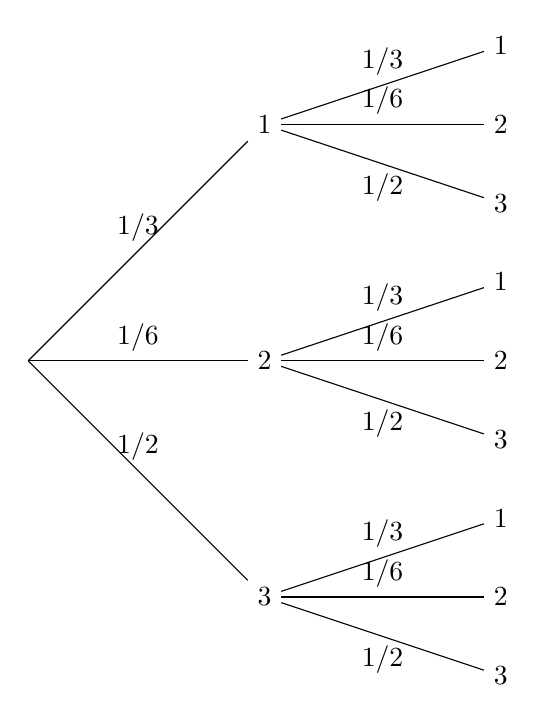
\begin{tikzpicture}
					      \coordinate (START) at (0,0);
					      \node (First1) at (3,3) {$1$};
					      \node (First2) at (3,0) {$2$};
					      \node (First3) at (3,-3) {$3$};

					      \foreach \n/\p in {First1/${1/3}$,First2/${1/6}$,First3/${1/2}$} {
							      \draw (START) -- node[above] {\p} (\n);
							      \node (Second1) at ($(\n) + (3,1)$) {$1$};
							      \node (Second2) at ($(\n) + (3,0)$) {$2$};
							      \node (Second3) at ($(\n) + (3,-1)$) {$3$};
							      \draw (\n) -- node[above] {$1/3$} (Second1);
							      \draw (\n) -- node[above] {$1/6$} (Second2);
							      \draw (\n) -- node[below] {$1/2$} (Second3);
						      }
				      \end{tikzpicture}
			      \end{center}
			\item La probabilité d'obtenir un $1$ au premier lancé et un $3$ au deuxième lancé est

			      $$ \dfrac{1}{3} × \dfrac{1}{2} = \dfrac{1}{6} $$
			\item Les issues donnant au moins un $2$ sur les deux lancés sont : $(1 ; 2)$, $(2 ; 1)$, $(2 ; 2)$, $(2 ; 3)$, $(3 ; 2)$.

			      La probabilité est donc

			      $$ \dfrac{1}{3} × \dfrac{1}{6} + \dfrac{1}{6} × \dfrac{1}{3} + \dfrac{1}{6} × \dfrac{1}{6} + \dfrac{1}{6} × \dfrac{1}{2} + \dfrac{1}{2} × \dfrac{1}{6} = \dfrac{11}{36} $$
		\end{enumerate}
	\end{multicols}
\end{exercice}

\begin{exercice}
	\begin{enumerate}
		\item \
		      \begin{center}
			      \begin{tabular}{|l|*{3}{>{\centering}p{2cm}|}}
				      \hline
				      \diagbox{Traitement}{Succès} & Réussi             & Échoue             & TOTAL \tabularnewline \hline
				      Traitement $A$               & \correction{$130$} & \correction{$10$}  & \correction{$140$} \tabularnewline \hline
				      Traitement $B$               & \correction{$390$} & \correction{$20$}  & \correction{$410$} \tabularnewline \hline
				      Traitement $C$               & \correction{$340$} & \correction{$110$} & \correction{$450$} \tabularnewline \hline
				      TOTAL                        & \correction{$860$} & \correction{$140$} & \correction{$1000$} \tabularnewline \hline
			      \end{tabular}
		      \end{center} \bigskip
		\item $P(C ∩ E) = \dfrac{110}{1000} = 0,11$ et $P(A ∩ R) = \dfrac{130}{1000} = 0,13$.
		\item Le traitement $A$ a $\dfrac{130}{140} ≈ 93\%$ de chances de réussite ;

		      Le traitement $B$ a $\dfrac{390}{410} ≈ 95\%$ de chances de réussite ;

		      Le traitement $C$ a $\dfrac{340}{450} ≈ 75\%$ de chances de réussite.

		      Le traitement $B$ semble donc meilleur.
	\end{enumerate}
\end{exercice}

%===============================================
%================== SUJET B ====================
%===============================================

\newpage\setcounter{exercice}{1}
\title{Évaluation probabilités (sujet B)}
\maketitle

\begin{exercice}
	\begin{enumerate}
		\item Compléter les phrases suivantes :
		      \begin{itemize}
			      \item $\overline{A}$ est l'évènement \correctionDots{contraire} de $A$.
			      \item $A ∩ B$ est l'évènement $A$ \correctionDots{ET} $B$.
			      \item $A ∪ B$ est l'évènement $A$ \correctionDots{ou} $B$.
		      \end{itemize}
		\item Si on sait que $P(A) = 0,5$, $P(B) = 0,4$ et $P(A ∩ B) = 0,2$, quelle est la probabilité de $A ∪ B$ ? {\color{red}$0,7$}
	\end{enumerate}
\end{exercice}

\begin{exercice}
	\begin{multicols}{2}
		\begin{enumerate}
			\item \
			      \begin{center}
				      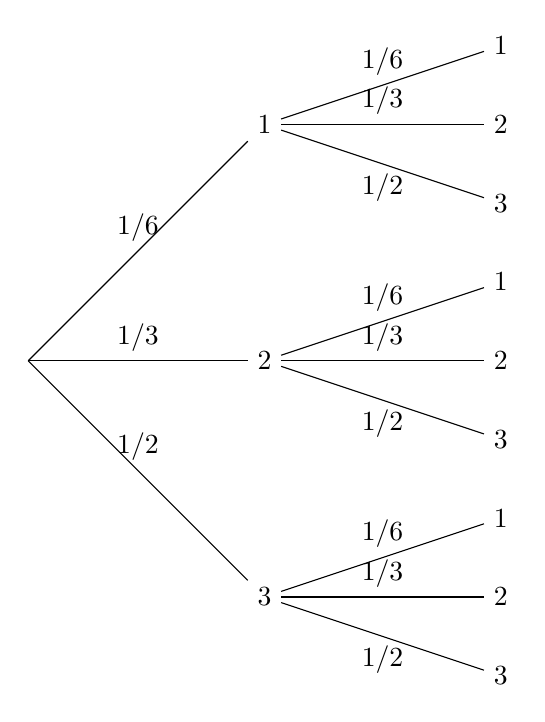
\begin{tikzpicture}
					      \coordinate (START) at (0,0);
					      \node (First1) at (3,3) {$1$};
					      \node (First2) at (3,0) {$2$};
					      \node (First3) at (3,-3) {$3$};

					      \foreach \n/\p in {First1/${1/6}$,First2/${1/3}$,First3/${1/2}$} {
							      \draw (START) -- node[above] {\p} (\n);
							      \node (Second1) at ($(\n) + (3,1)$) {$1$};
							      \node (Second2) at ($(\n) + (3,0)$) {$2$};
							      \node (Second3) at ($(\n) + (3,-1)$) {$3$};
							      \draw (\n) -- node[above] {$1/6$} (Second1);
							      \draw (\n) -- node[above] {$1/3$} (Second2);
							      \draw (\n) -- node[below] {$1/2$} (Second3);
						      }
				      \end{tikzpicture}
			      \end{center}
			\item La probabilité d'obtenir un $1$ au premier lancé et un $3$ au deuxième lancé est

			      $$ \dfrac{1}{6} × \dfrac{1}{2} = \dfrac{1}{12} $$
			\item Les issues donnant au moins un $2$ sur les deux lancés sont : $(1 ; 2)$, $(2 ; 1)$, $(2 ; 2)$, $(2 ; 3)$, $(3 ; 2)$.

			      La probabilité est donc

			      $$ \dfrac{1}{6} × \dfrac{1}{3} + \dfrac{1}{3} × \dfrac{1}{6} + \dfrac{1}{3} × \dfrac{1}{3} + \dfrac{1}{3} × \dfrac{1}{2} + \dfrac{1}{2} × \dfrac{1}{3} = \dfrac{5}{9} $$
		\end{enumerate}
	\end{multicols}
\end{exercice}

\begin{exercice}
	\begin{enumerate}
		\item \
		      \begin{center}
			      \begin{tabular}{|l|*{3}{>{\centering}p{2cm}|}}
				      \hline
				      \diagbox{Traitement}{Succès} & Réussi             & Échoue             & TOTAL \tabularnewline \hline
				      Traitement $A$               & \correction{$120$} & \correction{$10$}  & \correction{$130$} \tabularnewline \hline
				      Traitement $B$               & \correction{$400$} & \correction{$30$}  & \correction{$430$} \tabularnewline \hline
				      Traitement $C$               & \correction{$330$} & \correction{$110$} & \correction{$440$} \tabularnewline \hline
				      TOTAL                        & \correction{$850$} & \correction{$150$} & \correction{$1000$} \tabularnewline \hline
			      \end{tabular}
		      \end{center} \bigskip
		\item $P(A ∩ E) = \dfrac{10}{1000} = 0,01$ et $P(C ∩ R) = \dfrac{330}{1000} = 0,33$.
		\item Le traitement $A$ a $\dfrac{120}{130} ≈ 92\%$ de chances de réussite ;

		      Le traitement $B$ a $\dfrac{400}{430} ≈ 93\%$ de chances de réussite ;

		      Le traitement $C$ a $\dfrac{330}{440} = 75\%$ de chances de réussite.

		      Le traitement $B$ semble donc meilleur.
	\end{enumerate}
\end{exercice}

\end{document}